% =====================================================================
% Snippet: formula-box.tex
% =====================================================================
% USAGE: Formula box with title + math content + optional annotation.
% Three variants demoed below. Copy whichever fits, then replace:
%   - title: bold header above formula
%   - math: LaTeX math expression (use $...$ or \[...\])
%   - annotation: small italic explanation below (optional)
%   - origin_x, origin_y
%   - color: line + accent (use palette colors)
%
% Why use this snippet:
%   - Philosophy 段 "公式嵌入 = box 内部"，不是只贴 "FFN" 标签
%   - 例如 "FFN(x) = max(0, xW₁+b₁)W₂+b₂" 完整数学
% =====================================================================

\documentclass[tikz,border=10pt]{standalone}
\usepackage{xcolor,tikz,amsmath,amssymb}
\usetikzlibrary{positioning,calc}

\definecolor{acaPurpleLine}{HTML}{6E3FA0}
\definecolor{acaPurpleBg}{HTML}{EDE3F6}
\definecolor{acaOrangeLine}{HTML}{D06020}
\definecolor{acaOrangeBg}{HTML}{F9E0D0}
\definecolor{acaTealLine}{HTML}{1F8F8F}
\definecolor{acaTealBg}{HTML}{D3EBEB}
\definecolor{acaGreyLine}{HTML}{606060}

\tikzset{
  formula box/.style={
    rectangle, rounded corners=3pt,
    line width=0.6pt,
    inner sep=6pt,
    align=center,
  },
}

\begin{document}
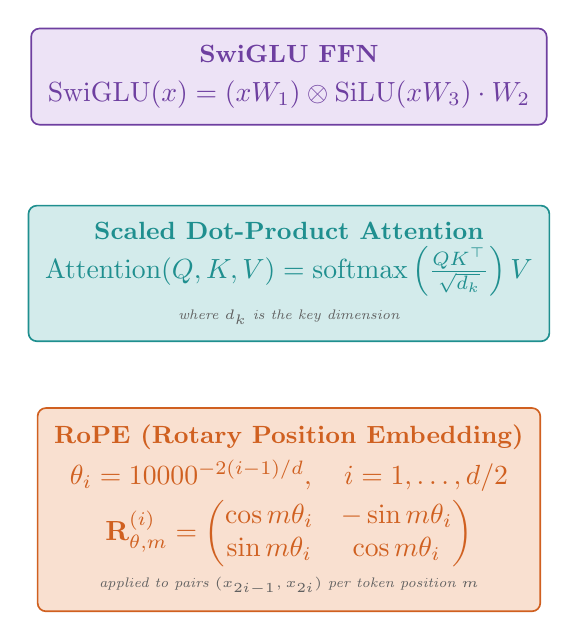
\begin{tikzpicture}

%% COPY-START (Variant A — Simple) ===================================
% Title + formula only
\node[formula box, fill=acaPurpleBg, draw=acaPurpleLine, text=acaPurpleLine]
  at (0, 0) {%
    {\small\bfseries SwiGLU FFN}\\[2pt]
    $\text{SwiGLU}(x) = (xW_1) \otimes \text{SiLU}(xW_3) \cdot W_2$
  };
%% COPY-END Variant A ================================================

%% COPY-START (Variant B — With annotation) ==========================
\node[formula box, fill=acaTealBg, draw=acaTealLine, text=acaTealLine]
  at (0, -2.5) {%
    {\small\bfseries Scaled Dot-Product Attention}\\[2pt]
    $\text{Attention}(Q, K, V) = \text{softmax}\left(\frac{QK^\top}{\sqrt{d_k}}\right) V$\\[3pt]
    {\tiny\itshape \color{acaGreyLine}where $d_k$ is the key dimension}
  };
%% COPY-END Variant B ================================================

%% COPY-START (Variant C — Multi-line derivation) ====================
\node[formula box, fill=acaOrangeBg, draw=acaOrangeLine, text=acaOrangeLine]
  at (0, -5.5) {%
    {\small\bfseries RoPE (Rotary Position Embedding)}\\[3pt]
    $\theta_i = 10000^{-2(i-1)/d}, \quad i = 1, \ldots, d/2$\\[2pt]
    $\mathbf{R}_{\theta,m}^{(i)} =
      \begin{pmatrix} \cos m\theta_i & -\sin m\theta_i \\
                      \sin m\theta_i &  \cos m\theta_i \end{pmatrix}$\\[3pt]
    {\tiny\itshape \color{acaGreyLine} applied to pairs $(x_{2i-1}, x_{2i})$ per token position $m$}
  };
%% COPY-END Variant C ================================================

\end{tikzpicture}
\end{document}
